\documentclass[]{default}
\usepackage{lmodern}
\usepackage{listings}
\usepackage{amssymb,amsmath}
\usepackage{paralist}
\usepackage{tikz-qtree}
\usepackage{enumitem}
\usepackage{ifxetex,ifluatex}
\usepackage{fixltx2e} % provides \textsubscript
\ifnum0\ifxetex{1}\fi\ifluatex{1}\fi=0 % if pdftex
  \usepackage[T1]{fontenc}
  \usepackage[utf8]{inputenc}
\else % if luatex or xelatex
  \ifxetex{
    \usepackage{mathspec}
    \usepackage{xltxtra,xunicode}
  \else
    \usepackage{fontspec}
  }\fi
  \defaultfontfeatures{Mapping=tex-text,Scale=MatchLowercase}
  \newcommand{\euro}{€}
\fi
% use upquote if available, for straight quotes in verbatim environments
\IfFileExists{upquote.sty}{\usepackage{upquote}}{}
% use microtype if available
\IfFileExists{microtype.sty}{%
\usepackage{microtype}
\UseMicrotypeSet[protrusion]{basicmath} % disable protrusion for tt fonts
}{}
\ifxetex%
  \usepackage[setpagesize=false, % page size defined by xetex
              unicode=false, % unicode breaks when used with xetex
              xetex]{hyperref}
\else
  \usepackage[unicode=true]{hyperref}
\fi
\hypersetup{breaklinks=true,
            bookmarks=true,
            pdfauthor={},
            pdftitle={Quantitative Benchmarks for Theory Exploration},
            colorlinks=true,
            citecolor=blue,
            urlcolor=blue,
            linkcolor=magenta,
            pdfborder={0 0 0}}
\urlstyle{same}  % don't use monospace font for urls
\setlength{\parindent}{0pt}
\setlength{\parskip}{6pt plus 2pt minus 1pt}
\setlength{\emergencystretch}{3em}  % prevent overfull lines
\setcounter{secnumdepth}{5}

\newcommand{\name}[1]{\mathrm{#1}}

\newcommand{\feature}[1]{\phi(#1)}
\newcommand{\id}[1]{\texttt{``#1''}}
\newcommand{\CVar}{\texttt{Var}}
\newcommand{\CLit}{\texttt{Lit}}
\newcommand{\CApp}{\texttt{App}}
\newcommand{\CLam}{\texttt{Lam}}
\newcommand{\CLet}{\texttt{Let}}
\newcommand{\CCase}{\texttt{Case}}
\newcommand{\CType}{\texttt{Type}}
\newcommand{\CLocal}{\texttt{Local}}
\newcommand{\CGlobal}{\texttt{Global}}
\newcommand{\CConstructor}{\texttt{Constructor}}
\newcommand{\CLitNum}{\texttt{LitNum}}
\newcommand{\CLitStr}{\texttt{LitStr}}
\newcommand{\CAlt}{\texttt{Alt}}
\newcommand{\CDataAlt}{\texttt{DataAlt}}
\newcommand{\CLitAlt}{\texttt{LitAlt}}
\newcommand{\CDefault}{\texttt{Default}}
\newcommand{\CNonRec}{\texttt{NonRec}}
\newcommand{\CRec}{\texttt{Rec}}
\newcommand{\CBind}{\texttt{Bind}}

\setlength{\belowcaptionskip}{-10pt}

\newlist{inlinelist}{enumerate*}{1}
\setlist*[inlinelist,1]{%
  label= (\roman*),
}

\title{Quantitative Benchmarks for Theory Exploration}
  \author{Chris Warburton \\
          University of Dundee \\
          \texttt{cmwarburton@dundee.ac.uk}}
\date{}

\begin{document}
\maketitle
\begin{abstract}
  \emph{Automated theory exploration} has the potential to help scientists,
  mathematicians and programmers discover unexpected properties of their models,
  theories and programs; but has so far been limited to small-scale experiments,
  with only a few, hand-picked, data points. We address this problem by
  re-purposing existing benchmarks from the theorem proving domain, producing an
  order of magnitude more data for evaluation, and use it to evaluate the
  performance of a state of the art exploration system. To combat the long run
  times of these systems, we also propose a pre-processing method to identify
  promising subsets of a theory, sacrificing completeness to gain speed. It is
  our hope that the availability of robust evaluation methods, and scalable
  algorithms, will encourage competition and innovation, making theory
  exploration more useful and relevant in formal methods.
\end{abstract}

%\vspace{-2mm}

\textbf{Keywords:} Theory exploration, automated reasoning, automated theorem
proving

%\vspace{-2mm}

\section{Introduction}\label{introduction}

Many fields represent knowledge using \emph{formal systems}, for example
scientific models, mathematical theories and computer programs. These systems
can be extended to meet new demands in two ways: the systems can be made more
complex, or many new systems can be defined. Complexification makes a system's
behaviour harder to predict, whilst proliferation dilutes the attention that can
be given to each particular system. This presents a challenge for experts
needing to characterise the behaviour of such systems, for example to prove
properties related to protocol security or mechanical safety.

One way to help these experts is through automation: formal systems are easily
represented as software, and techniques like \emph{automated theory exploration}
can help experts to discover properties of a system, whether expected or
surprising, desirable or not.

\vspace{-2mm}

\section{Background}\label{background}

An example of a simple formal system is the following software
library:

\vspace{-5mm}

\begin{equation*}
  \begin{aligned}
    \name{append}(\name{nil},        z) &= z                                   \\
    \name{append}(\name{cons}(x,y),  z) &= \name{cons}(x, \name{append}(y, z)) \\
    \name{map}(f,           \name{nil}) &= \name{nil}                          \\
    \name{map}(f,    \name{cons}(x, y)) &= \name{cons}(f(x), \name{map}(f, y))
  \end{aligned}
\end{equation*}

These equations define two functions, $\name{append}$ (for joining one list to
another) and $\name{map}$ (for applying a function to the elements of a list),
based on the way they rearrange particular constants ($\name{nil}$ and
$\name{cons}$, which encode lists à la Lisp) and variables ($f$, $x$, $y$, $z$).
One \emph{property} of this library is that the following expressions are
equivalent:

\vspace{-3mm}

\begin{equation}\label{eq:mapappend}
  \name{map}(f, \name{append}(x, y)) =
    \name{append}(\name{map}(f, x), \name{map}(f, y))
\end{equation}

This states that $\name{map}$ distributes over $\name{append}$, i.e.\ we can
perform $\name{map}$ and $\name{append}$ in either order and get the same
result. This is useful, since it may be much faster to run $\name{map}(f, x)$
and $\name{map}(f, y)$ in parallel on different machines, then $\name{append}$
the results; compared to $\name{append}$ing the inputs and running one big
$\name{map}$.\footnote{This is one half of the ``MapReduce'' model for parallel
  programming.~\cite{dean2008mapreduce}.}

Most automation of formal systems focuses on \emph{automated theorem proving}
(ATP), which dates back to the early days of artificial
intelligence~\cite{newell1956logic}. In ATP, the user gives a particular
property statement (like \ref{eq:mapappend}) to the program up front, and the
program searches for a proof. Modern ATP systems, such as
CVC4~\cite{barrett2011cvc4}, compete regularly to prove as many benchmark
problems as they can, as quickly as possible~\cite{sutcliffe2006state}.

\emph{Automated Theory Exploration} (ATE) is the task of taking in a formal
system (such as the definitions of $\name{map}$ and $\name{append}$ above) and
giving out interesting properties, like \ref{eq:mapappend}.\footnote{ATE doesn't
  require a proof of these properties; we can use ATP tools for that.} ATE has
seen little attention, partly because of its resource usage, and partly because
it is difficult to evaluate: what makes a property ``interesting''? Many general
measures have been proposed\cite{colton2000notion}, but for comparison purposes
we can stick to known theories and simply check if a human has bothered to state
these properties before!

Existing ATE programs such as \textsc{QuickSpec}~\cite{QuickSpec} and
\textsc{IsaCoSy}~\cite{johansson2009isacosy} have been evaluated this way on
theories of lists and natural numbers taken from the Isabelle proof
assistant~\cite{claessen2013automating}. The discovered properties are compared
against those in Isabelle, to see how many match up. Unfortunately these are the
only data sets used, and each is rather small (containing 9 and 12 properties,
respectively). This is not enough data from which to draw meaningful comparisons
or extrapolations.

\section{Contributions}

\subsection{Benchmarking}

We address the problem of ATE evaluation by implementing a much larger benchmark
suite, containing 343 properties of 269 definitions. We take these from an
existing ATP benchmark called TIP\cite{claessen2015tip}, since it
\begin{inlinelist}
\item separates definitions from theorems
\item allows higher-order functions (like $\name{map}$)
\item incorporates many tricky problems from the theorem-proving literature
\item contains problems of immediate relevance to software verification
\end{inlinelist}.

Each TIP property is given alongside all of its required definitions. We
re-purpose these for the ATE setting, by pooling together all of
the definitions\footnote{Including custom functions to construct and destruct
  constant values (like $\name{nil}$ and $\name{cons}$), we get 3595
  definitions, most of which are redundant copies used in many problems.
  Discarding these leaves 269 distinct definitions.} and all of the properties.

We provide a tool to sample subsets of these definitions, along with the subset
of properties which apply to that sample, so that theories of various sizes can
be generated for evaluating ATE systems.

\subsection{Scaling}\label{recurrent-clustering}

In the worst case, ATE scales exponentially with the number of definitions in a
theory. We have also investigated ways to mitigate this using \emph{relevance
  filtering}~\cite{meng2009lightweight}: given a large theory, can we explore
only those definitions which we expect to yield interesting properties? We have
implemented such a filter based on
\emph{recurrent clustering}~\cite{journals/corr/abs-1212-3618}, which compares
the syntax trees of a theory's definitions to find those which are similar. We
have also made a purely random filter, to control for the effect of
\emph{filtering itself}. These can be used as a pre-processor for any ATE system
and work is ongoing to evaluate their effect on property recall and performance.

\section{Results}

\begin{figure}
  \centering
  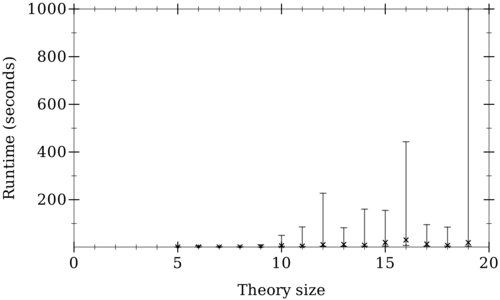
\includegraphics[width=0.45\textwidth]{runtimes}
  \vspace{-3mm}
  \caption{Median runtime of the \textsc{QuickSpec} ATE system for 30 iterations
    on theories of various size, sampled from TIP. Error bars show the
    interquartile range. We time out at 1000 seconds.}\label{fig:runtimes}
  \vspace{-5mm}
\end{figure}

Figure~\ref{fig:runtimes} shows the median run time of \textsc{QuickSpec} as we
explore theories of various size sampled from our benchmark. We have found that
the time taken can vary greatly, even among theories of the same size, with most
finishing after a few seconds but some taking hours; this can be seen by the
increase in range for larger theories, despite the median remaining low.

This variance makes current ATE systems inconvenient for widespread use. Finding
a pattern in these long-running inputs is current work; our hope is that
approaches like our relevance filter make ATE more predictable and tractable.

\section{Future Work}\label{future-work}

There are many promising directions that this work enables. Our benchmark is
currently limited to ATE systems using Haskell; integrating other languages
would allow wider comparisons, e.g. to IsaCoSy and IsaScheme which use Isabelle.

Machine learning is a promising direction for scaling ATE, since its approximate
methods may be more efficient than existing searches, and its data-driven
approach is well suited to handle fuzzy concepts such as ``interestingness''.
Our benchmark can act as both a fitness function and a training corpus for such
efforts.

Our system can explore \emph{arbitrary} code, not just our benchmarks. Besides
listing properties, potential applications include tools for optimisation (if
coupled to a profiler) and refactoring (e.g. using properties to propose new
abstractions).

\bibliographystyle{plain}
\bibliography{./Bibtex}

\end{document}
